\section{Auswertung}

\subsection{Lichtgeschwindigkeitsmessung}

\begin{table}[H]
    \caption{Distanzmessungen bei Inkrementieren und Dekrementieren der Drehfrequenz}
    \begin{subtable}{.5\linewidth}
        \centering
        \caption{Messung von Alex Murray}
        \label{tab:am-f-x}
        \begin{tabular}{cc}
            \toprule
            Drehfrequenz ($Hz$) & Distanz ($\mu m$) \\
            \midrule
            498  & 0    \\
            605  & -83  \\
            702  & -169 \\
            800  & -250 \\
            885  & -324 \\
            1008 & -414 \\
            1096 & -499 \\
            1200 & -586 \\
            1305 & -666 \\
            1400 & -741 \\
            1498 & -839 \\
            \bottomrule
        \end{tabular}
    \end{subtable}
    \begin{subtable}{.5\linewidth}
        \centering
        \caption{Messung von Yohannes Measho}
        \label{tab:ym-f-x}
        \begin{tabular}{cc}
            \toprule
            Drehfrequenz ($Hz$) & Distanz ($\mu m$) \\
            \midrule
            1498 & 0   \\
            1388 & 124 \\
            1289 & 192 \\
            1199 & 280 \\
            1106 & 353 \\
            1009 & 431 \\
            912  & 516 \\
            807  & 590 \\
            708  & 682 \\
            603  & 771 \\
            502  & 851 \\
            \bottomrule
        \end{tabular}
    \end{subtable}
\end{table}

In den Tabellen \ref{tab:am-f-x} und  \ref{tab:ym-f-x}  sind die von Alex Murray
und   Yohannes   Measho   gemessene  Distanzenverschiebungen  in  Funktion   der
Drehfrequenz  $f$  aufgezeichnet.  Die Messungen in der Tabelle \ref{tab:am-f-x}
wurden bei Inkrementieren der Drehfrequenz erfasst, die Messungen in der Tabelle
\ref{tab:ym-f-x}   wurden   bei   Dekrementieren   der   Drehfrequenz   erfasst.

\begin{figure}[H]
    \center
    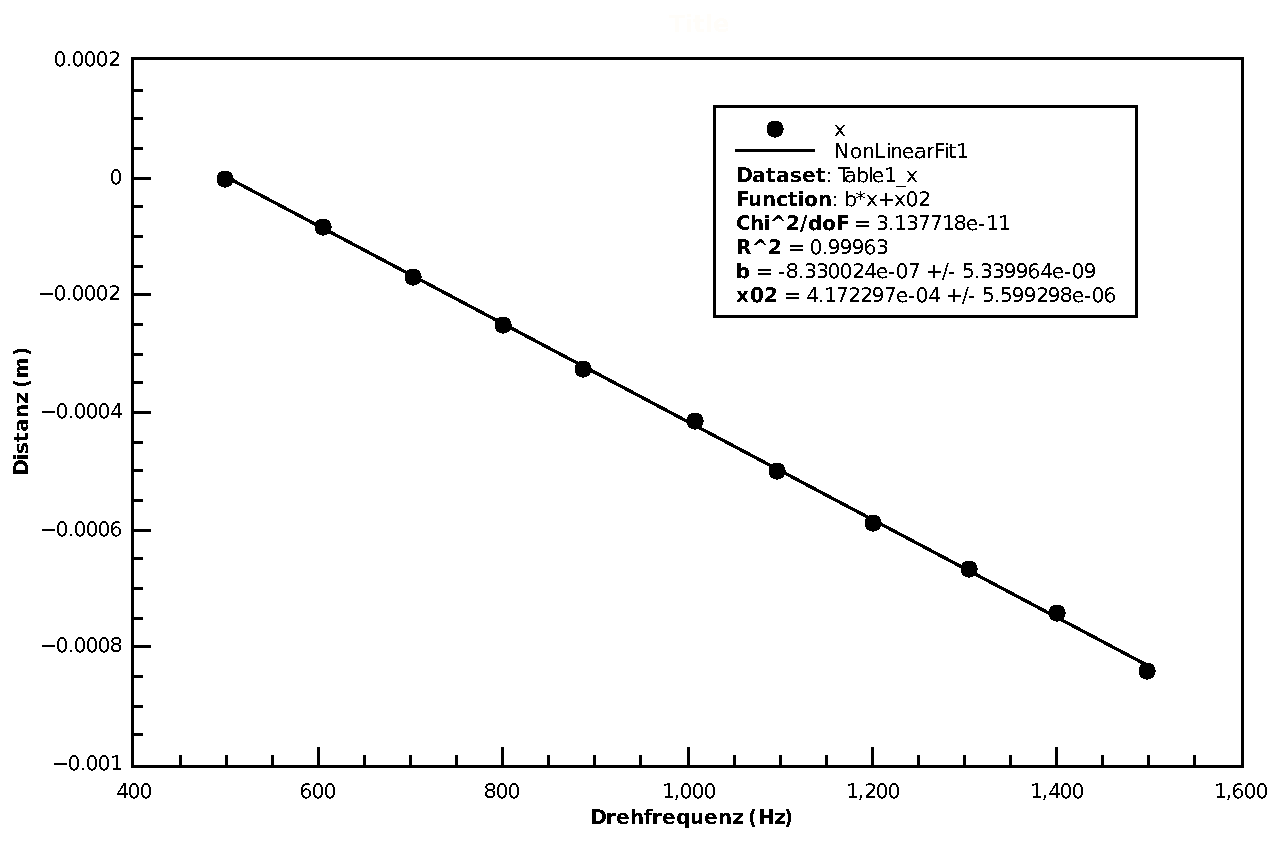
\includegraphics[width=.8\textwidth]{images/am-f-x-fit-b.pdf}
    \caption{Lineare Regression zur Berechnung des Faktors $b$, Messdaten von Alex Murray}
    \label{fig:am-f-x-fit-b}
\end{figure}

In  der Abbildung \ref{fig:am-f-x-fit-b} sind die  Messpunkte  von  der  Tabelle
\ref{tab:am-f-x} als  XY-Scatter  Plot  dargestellt.  Die Punkte wurden nach der
Formel \ref{eq:lichtgeschwindigkeit} gefittet und damit ergibt  sich  der Faktor
$b_{Alex}$ als:
\begin{equation}
    b_{Alex} = \overline{b_{Alex}} \pm s_{\overline{b_{Alex}}} = -(833.0024 \pm 5.3400)\cdot 10^{-9}
    \label{eq:am-b}
\end{equation}

\begin{figure}[H]
    \center
    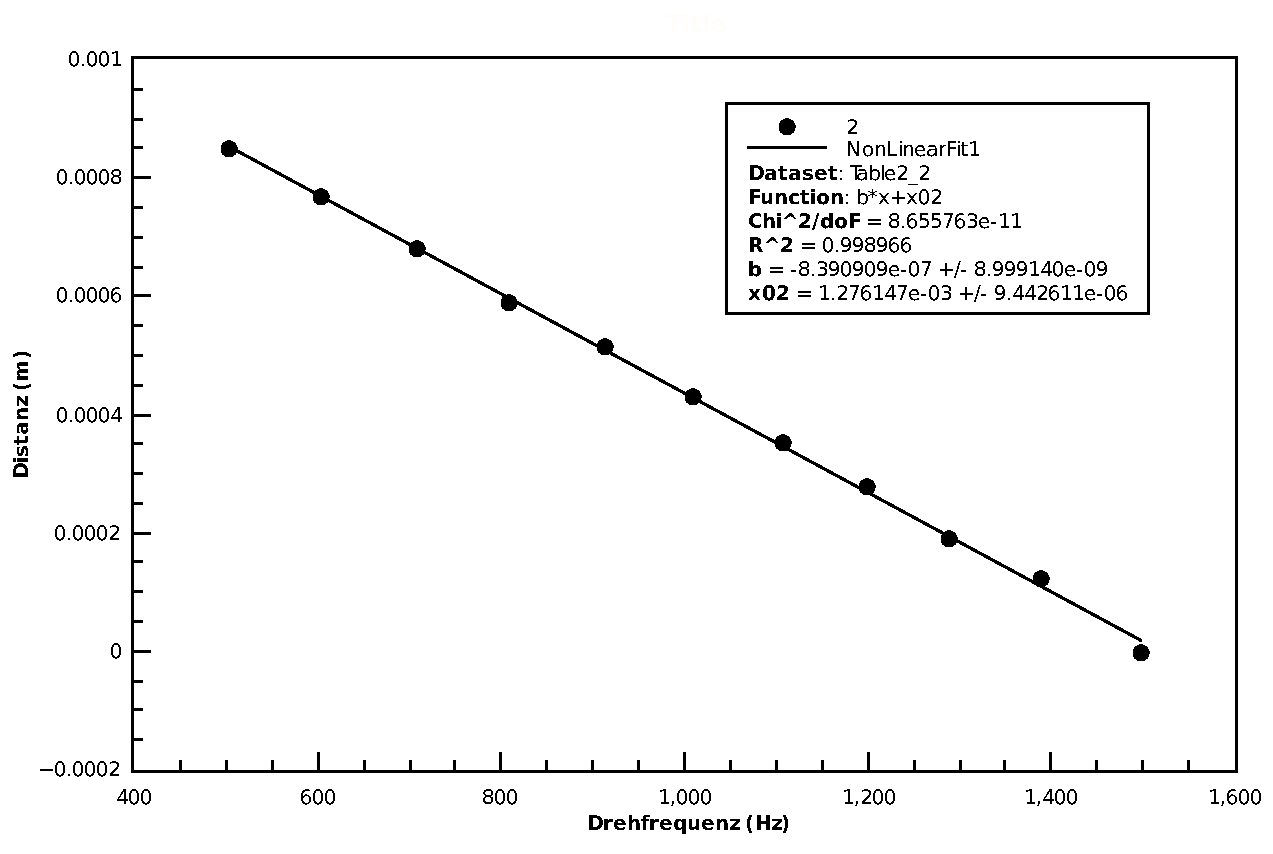
\includegraphics[width=.8\textwidth]{images/ym-f-x-fit-b.pdf}
    \caption{Lineare Regression zur Berechnung des Faktors $b$, Messdaten von Yohannes Measho}
    \label{fig:ym-f-x-fit-b}
\end{figure}

In der Abbildung \ref{fig:ym-f-x-fit-b} sind  die  Messpunkte  von  der  Tabelle
\ref{tab:ym-f-x}  als  XY-Scatter  Plot  dargestellt. Die Punkte wurden nach der
Formel \ref{eq:lichtgeschwindigkeit} gefittet und damit ergibt sich  der  Faktor
$b_{Yohannes}$ als:
\begin{equation}
    b_{Yohannes} = \overline{b_{Yohannes}} \pm s_{\overline{b_{Yohannes}}} = -(839.0909 \pm 8.9991)\cdot 10^{-9}
    \label{eq:ym-b}
\end{equation}


\subsection{Kalibrationsmessung}

\begin{table}[H]
    \caption{Kalibrationsmessdaten}
    \begin{subtable}{.5\linewidth}
        \centering
        \caption{Messung von Alex Murray}
        \label{tab:am-x-z}
        \begin{tabular}{ccc}
            \toprule
            $x (mm)$ & \hspace{5mm} & $z (mm)$ \\
            \midrule
            10.042 && 12.5 \\
            8.031  && 13.0 \\
            6.049  && 13.5 \\
            4.049  && 14.0 \\
            1.990  && 14.5 \\
            -0.019 && 15.0 \\
            -1.988 && 15.5 \\
            -3.955 && 16.0 \\
            -5.954 && 16.5 \\
            -7.973 && 16.5 \\
            -9.952 && 17.5 \\
            \bottomrule
        \end{tabular}
    \end{subtable}%
    \begin{subtable}{.5\linewidth}
        \centering
        \caption{Messung von Yohannes Measho}
        \label{tab:ym-x-z}
        \begin{tabular}{ccc}
            \toprule
            $x (mm)$ & \hspace{5mm} & $z (mm)$ \\
            \midrule
            10.047 && 12.5 \\
            8.020  && 13.0 \\
            5.980  && 13.5 \\
            3.990  && 14.0 \\
            1.926  && 14.5 \\
            -0.053 && 15.0 \\
            -2.048 && 15.5 \\
            -4.030 && 16.0 \\
            -6.039 && 16.5 \\
            -7.997 && 17.0 \\
            -9.987 && 17.5 \\
           \bottomrule
        \end{tabular}
    \end{subtable}
\end{table}

In    den   Tabellen   \ref{tab:am-x-z}   und    \ref{tab:ym-x-z}    sind    die
Kalibrationsmessungen von Alex Murray  und  Yohannes  Measho aufgef\"uhrt. Beide
haben   die   gleiche   Messung   unabh\"angig  von   einander   durchgef\"uhrt.

\begin{figure}[H]
    \center
    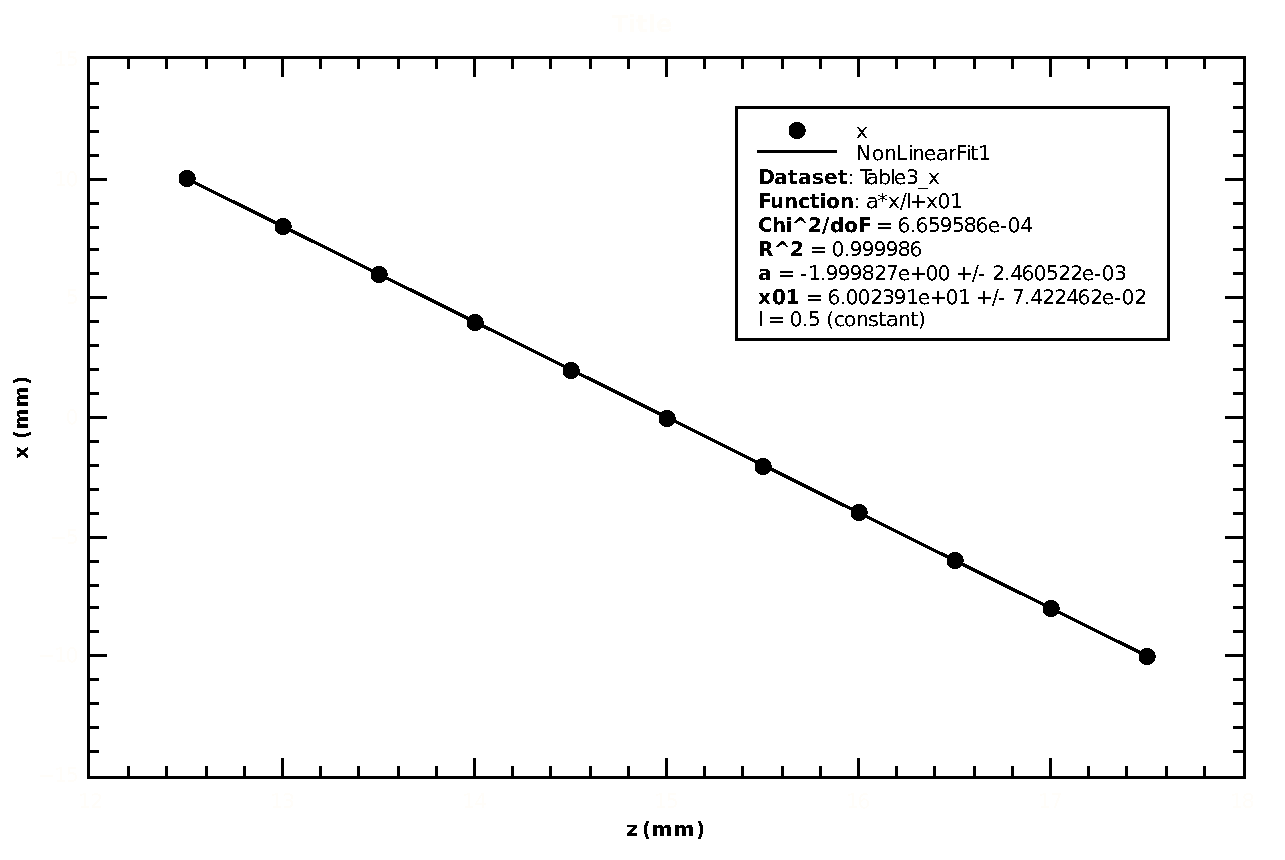
\includegraphics[width=.8\textwidth]{images/am-x-z-fit-a.pdf}
    \caption{Lineare Regression zur Berechnung des Faktors $a$ anhand der Kalibrationsmessung, Messdaten von Alex Murray}
    \label{fig:am-x-z-fit-a}
\end{figure}

In der Abbildung \ref{fig:am-x-z-fit-a}  sind  die  Messpunkte  von  der Tabelle
\ref{tab:am-x-z} als XY-Scatter Plot dargestellt.  Die  Punkte  wurden  nach der
Formel  \ref{eq:kalibration-a}   gefittet  und  somit  ergibt  sich  der  Faktor
$a_{Alex}$ als:
\begin{equation}
    a_{Alex} = \overline{a_{Alex}} \pm s_{\overline{a_{Alex}}} = -(1999.827 \pm 2.461)\cdot 10^{-3}
    \label{eq:am-a}
\end{equation}

\begin{figure}[H]
    \center
    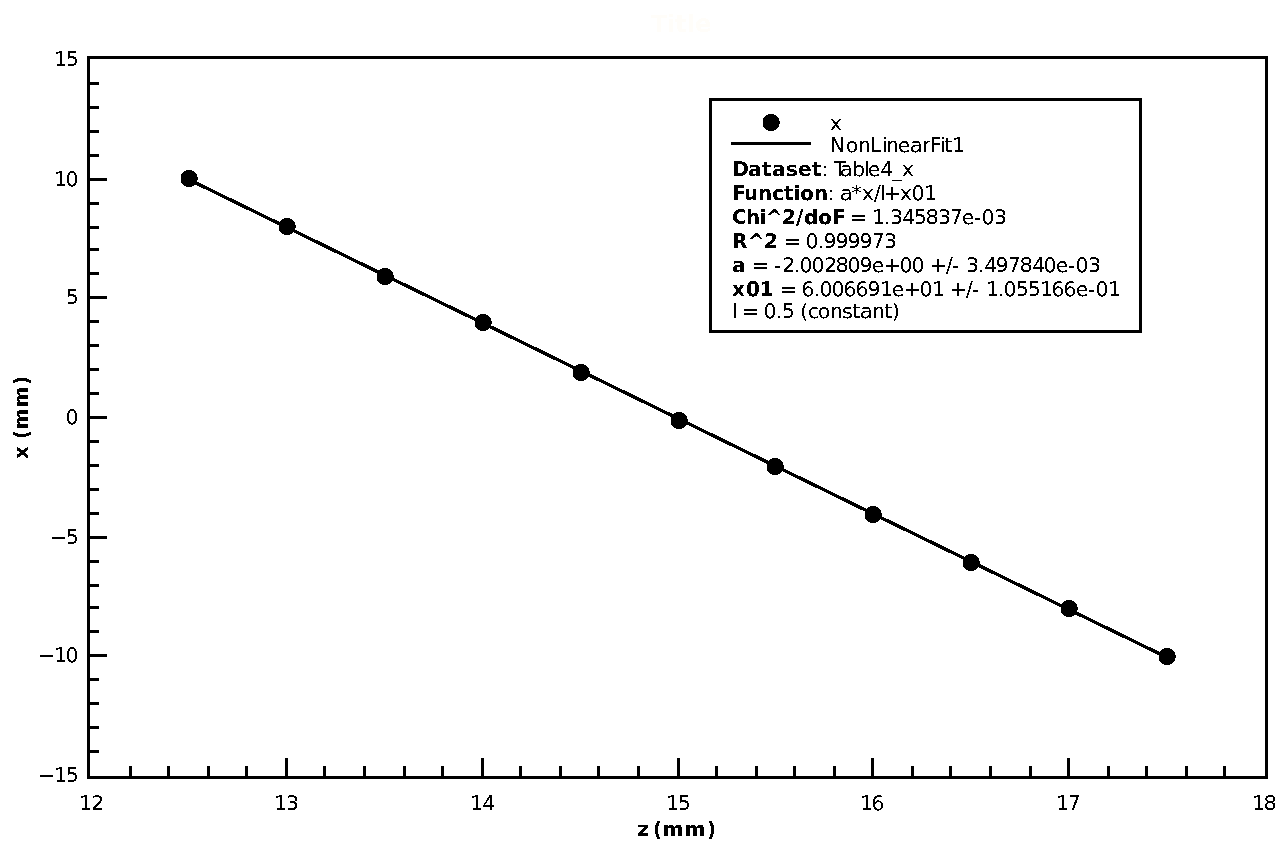
\includegraphics[width=.8\textwidth]{images/ym-x-z-fit-a.pdf}
    \caption{Lineare Regression zur Berechnung des Faktors $a$ anhand der Kalibrationsmessung, Messdaten von Yohannes Measho}
    \label{fig:ym-x-z-fit-a}
\end{figure}

In  der  Abbildung \ref{fig:ym-x-z-fit-a} sind die Messpunkte  von  der  Tabelle
\ref{tab:ym-x-z} als XY-Scatter Plot dargestellt. Die  Punkte  wurden  nach  der
Formel  \ref{eq:kalibration-a}   gefittet  und  somit  ergibt  sich  der  Faktor
$a_{Yohannes}$ als:
\begin{equation}
    a_{Yohannes} = \overline{a_{Yohannes}} \pm s_{\overline{a_{Yohannes}}} = -(2002.809 \pm 3.498)\cdot 10^{-3}
    \label{eq:ym-a}
\end{equation}
